\chapter{Problem Statement and Objectives}
\begin{justify}
    
\section{Problem Statement}
The current process for connecting influencers with brands in India remains disorganized and inefficient. Influencers often rely on informal methods such as direct social media messages to negotiate collaborations, which leads to frequent miscommunication, lack of transparency, and delayed payments. Furthermore, there is no standardized system for verifying influencers, which increases the risk of fraudulent profiles and wasted marketing budgets. Traditional communication channels do not provide a secure way to track task completion, making it difficult for brands to confirm that work has been done before payments are released.

Existing platforms for influencer marketing are either too generalized, leaving specific needs unmet, or too fragmented, with no central system to facilitate streamlined, trustworthy interactions between influencers and brands. This creates a significant gap in the influencer marketing ecosystem, one that hampers growth and reduces the overall effectiveness of digital campaigns. 
The current influencer-brand collaboration process in India is largely unstructured, informal, and prone to issues such as:
\begin{enumerate}
    \item Lack of a centralized and secure platform for verified influencer discovery.
    \item Frequent miscommunication between influencers and brands due to the absence of real-time collaboration tools.
    \item Non-transparent pricing models and payment terms.
    \item High risk of fraud and delayed or failed payments.
    \item Absence of project tracking and milestone management.
    \item Limited support for influencer-to-influencer collaboration.
\end{enumerate}
These issues not only hinder the efficiency and professionalism of digital marketing campaigns but also result in loss of trust between stakeholders.


\section{Project Objectives}

The primary aim of the Influencify platform is to address the challenges faced by influencers and brands in the current marketing ecosystem. By providing a secure, transparent, and efficient solution, the platform seeks to streamline the entire collaboration process. The project aims to improve communication, ensure fair payments, and create a centralized hub for verified influencers and brands to connect. The objectives of this project are designed to bridge the gaps in existing systems and promote a more reliable and organized approach to influencer marketing.

\begin{enumerate}
    \item 	\textbf{To connect verified Indian influencers and brands through a secure, centralized platform} that facilitates trusted and seamless collaboration. The platform will serve as a digital ecosystem where only authenticated influencers and legitimate clients can participate, thereby reducing the risks associated with fraudulent accounts, fake collaborations, and spam engagements.
    \item \textbf{To enable transparent pricing, direct communication, and comprehensive project tracking features} that ensure both parties have a clear understanding of deliverables, expectations, timelines, and payments. Influencers will be able to list their services with defined pricing packages, while brands can initiate discussions, negotiate deliverables, and track the status of campaigns in real time. These features are aimed at eliminating ambiguity and minimizing miscommunication throughout the collaboration process.
    \item \textbf{ To ensure timely and fair payments through the implementation of a milestone-based escrow system}, where payments from brands are securely held and released only upon successful completion and approval of predefined project stages. This objective aims to build financial trust, prevent payment fraud, and give both influencers and clients confidence in the collaboration process by offering clear terms, audit trails, and dispute resolution mechanisms.
    \item \textbf{	To promote influencer-to-influencer collaborations by creating a dedicated module or space within the platform} where creators can connect, pitch ideas, co-create content, and participate in joint campaigns. This feature will encourage networking, creative partnerships, and organic audience growth by allowing influencers to leverage each other’s strengths and reach, thereby enhancing community-driven content creation.
\end{enumerate}

\section{System Workflow Diagram}
\begin{figure}[H]
    \centering
    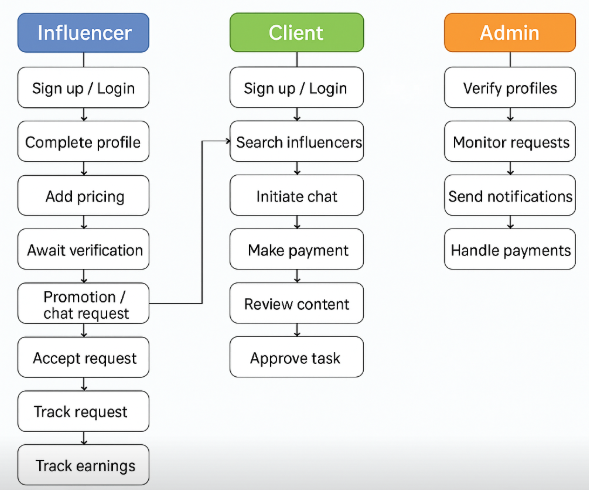
\includegraphics[height=0.5\textheight]{Chapters/Screenshot 2025-05-14 102150.png}
    \caption{System Workflow Diagram}
    \label{fig:system-workflow}
\end{figure}
  \end{justify}




